%! Author = sshcherbyna
%! Date = 24/06/2020

\documentclass{beamer}
\mode<presentation>
\hypersetup{pdfpagemode=FullScreen}
\usetheme{Warsaw}

\usepackage[utf8]{inputenc}
\usepackage{hyperref}
\usepackage[hyphenbreaks]{breakurl}
\usepackage{codeanatomy}
\usepackage{commutative-diagrams}
\usepackage{fontspec}
\usepackage{xcolor}
\usepackage{listings}
\usepackage[verbatim]{lstfiracode}
\setmonofont[Contextuals={Alternate}]{Fira Code}
\lstset{language=Scala,
style=FiraCodeStyle,
basicstyle=\ttfamily,
otherkeywords={},
columns = flexible,
mathescape}
\hypersetup{colorlinks,urlcolor=blue}
\urlstyle{sf}

\title{Delimited continuations as exponential objects}

\date{\today}
\author{Sergiy Shcherbyna}
\begin{document}
    \maketitle

    \begin{frame}[fragile]{Delimited continuations}
        \url{http://pllab.is.ocha.ac.jp/~asai/papers/pwl17.pdf}
        \begin{block}{Kenichi Asai. Delimited Continuations for Everyone}
            \begin{quote}
                \textbf{Are shift/reset really necessary?} \\
                They provide us with higher level of \alert{abstraction}.
            \end{quote}
            \begin{quote}
                We have a \alert{type system} for shift and reset, \\
                but their relationship to logic is \alert{unknown}.
            \end{quote}
            \begin{quote}
                Shift is \alert{intuitionistic}: even if we use shift, \\
                we cannot construct a term having a classic type.
            \end{quote}
        \end{block}
    \end{frame}

    \begin{frame}[fragile]{Delimited continuations}
        \begin{block}{The rest of the computation up to the delimiter}
            reset (fun () \rightarrow M)
        \end{block}
        \begin{definition}
            shift (fun k \rightarrow M)
            \begin{itemize}
                \item It clears the current continuation,
                \item binds the cleared continuation to k,
                \item and executes the body M in the empty context.
            \end{itemize}
        \end{definition}
    \end{frame}

    \begin{frame}[fragile]{Delimited continuations}
        \begin{example}
            \begin{lstlisting}
  def delay[A, B] (a: => A) =
    shift((k: A => B) => () => k(a) )

  val example1 = reset(for {
    _ <- delay(println("Hello,"))
    _ <- delay(println("World!"))
    _ <- delay(println("Goodbye!"))
  } yield ())
            \end{lstlisting}
        \end{example}
    \end{frame}

    \begin{frame}[fragile]{Delimited continuations}
        \begin{example}
            \begin{lstlisting}
  val example2 = reset(for {
    _ <- delay(println("1"))
    _ <- delay(println("2"))
    _ <- delay(println("3"))
    _ <- delay(println("4"))
  } yield ())

  def par[A1, A2] (
    t: (() => A1, () => A2)
  ): (A1, A2) = (t._1 (), t._2 () )
            \end{lstlisting}
        \end{example}
    \end{frame}

    \begin{frame}[fragile]{Delimited continuations}
        \begin{example}
            \begin{lstlisting}
par(par(par(example1, example2)))
            \end{lstlisting}
        \end{example}
        \begin{verbatim}
Hello,
1
World!
2
Goodbye!
3

Process finished with exit code 0
        \end{verbatim}
    \end{frame}

    \begin{frame}[fragile]{Delimited continuations in Scala}
        \url{https://dl.acm.org/doi/10.1145/1631687.1596596}
        \begin{block}{Authors: Tiark Rompf, Ingo Maier, Martin Odersky}
            Implementing first-class polymorphic delimited continuations
            by a type-directed selective CPS-transform
        \end{block}
        \begin{example}
            \begin{lstlisting}
val x = reset {
  shift { k: (Int=>Int) =>
    k(k(k(7))); "done"
  } + 1
}
println(x)
            \end{lstlisting}
            Output: done
        \end{example}
    \end{frame}

    \begin{frame}[fragile]{Delimited continuations in Scala}
        \begin{block}{Direct-Style Monads}
            Another interesting example is the use of monads in direct-style programming (Filinski 1994, 1999).
            As has been shown by Filinski, delimited continuations can express any definable monad.
        \end{block}
        \begin{example}
            \begin{lstlisting}
implicit class MonadReflect[+A,F[_]:Monad]
  (val xs: F[A]) extends AnyVal {
  def reflect[B](): A @cps[C[B], C[B]] =
    shift { k:(A => C[B]) => xs.flatMap(k) }
}
            \end{lstlisting}
        \end{example}
    \end{frame}

    \begin{frame}[fragile]{Delimited continuations in Scala}
        \begin{block}{Direct-Style Monads}
            The unit constructor List is used here as Filinski’s reify operation.
            The same mechanism applies to other monads, too.
        \end{block}
        \begin{example}
            \begin{lstlisting}
reset {
 List((
   List("x","y","z").reflect,
   List(4,5,6).reflect
 ))
}
            \end{lstlisting}
            result: cartesian product
            \begin{lstlisting}
List(("x",4), ("y","5"), ("z",6))
            \end{lstlisting}
        \end{example}
    \end{frame}

    \begin{frame}[fragile]{Delimited continuations in Scala}
        \begin{center}
            \begin{block}{String @cps[Int, List[Int]]}
                \url{https://stackoverflow.com/questions/17450444/scala-continuation-type-error}
            \end{block}
            \begin{example}
                \begin{lstlisting}
def f():Int @cpsParam[Int,Int] =
{shift { (k:Int=>Int) => k(6) } - 1}
<console>:4: error: type mismatch;
found: Int @scala.util.continuations.cpsSynth
@scala.util.continuations.cpsParam[Int,Int]
 required: Int
                \end{lstlisting}
            \end{example}
        \end{center}
    \end{frame}

    \begin{frame}[fragile]{Delimited continuations in Scala}
        \begin{alertblock}{Scala 2.13 support is missing}
            https://github.com/scala/scala-continuations/issues/37 \\
            \alert{Open} - SethTisue opened this issue on 29 Jan 2018
        \end{alertblock}
        \begin{block}{Odersky - SIP Committee member - Jul '19 }
            The continuations plugin was indeed discontinued because nobody was volunteering to maintain it.
            If people feel differently now, and have time to spend, it would be nice to restart the effort.\\
            \alert{\textbf{But it will be a lot of work.}}
        \end{block}
    \end{frame}

    \begin{frame}[fragile]{Delimited continuations in Scala}
        \begin{block}{Tiark Rompf, Ingo Maier, Martin Odersky.
        Implementing first-class polymorphic delimited continuations
        by a type-directed selective CPS-transform}
            Taking a step back, we consider how we might implement delimited continuations as \alert{user-level} Scala code.
            The technique we use comes as no surprise and is a straightforward generalization of the continuation monad
            to one that is parametric in the answer types. On a theoretical level, \alert{parameterized monads} have been
            studied in (Atkey 2006).
        \end{block}
    \end{frame}

    \begin{frame}[fragile]{Parameterized monads}
        \url{https://bentnib.org/paramnotions-jfp.html} \\
        Robert Atkey. Parameterised notions of computation. (2009)
        \begin{definition}
            Given a category C with finite products and a category S,
            an S-parameterised monad (T, \eta, \mu) on C consists of:
            \begin{itemize}
                \item A functor T : S\textsuperscript{op} × S × C → C;
                \item  A unit \eta\textsubscript{S,A} : A → T(S,S,A), natural in A and dinatural in S;
                \item  A multiplication \mu\textsubscript{S\textsubscript{1},S\textsubscript{2},S\textsubscript{3},A} : T(S\textsubscript{1},S\textsubscript{2},T(S\textsubscript{2},S\textsubscript{3},A)) → T(S\textsubscript{1},S\textsubscript{3},A), natural
                in S\textsubscript{1},S\textsubscript{3} and A and dinatural in S\textsubscript{2};
                \item  A strength \tau\textsubscript{A,S\textsubscript{1},S\textsubscript{2},B} : A × T(S\textsubscript{1},S\textsubscript{2},B) → T(S\textsubscript{1},S\textsubscript{2},A × B), natural in
                A,B,S\textsubscript{1} and S\textsubscript{2}.
            \end{itemize}
        \end{definition}
    \end{frame}

    \begin{frame}[fragile]{Parameterized monads}
        \begin{definition}
            An alternative partial definition is given by observing that a non-parameterised monad is equivalent to a one object C\textsuperscript{C}-enriched category. A multiple object C\textsuperscript{C} enriched category is equivalent to part of our definition, where the objects are the objects of the parameterising category S. Since a one object normal category
            is equivalent to a monoid, we can consider the relationship between parameterised monads and monads as similar to the relationship between monoids and categories. As a special case, if we restrict S to be the one object, one arrow category then our definition is equivalent to the standard definition of a non-parameterised monad.
        \end{definition}
        This observation is due to Chung-chieh Shan: \\
        \url{http://haskell.org/pipermail/haskell-cafe/2004-July/006448.html}
    \end{frame}

    \begin{frame}[fragile]{[Haskell-cafe] state in the continuation monad...}
        \begin{block}{On 2004-07-02T16:15:15+0200, Ralf Laemmel wrote}
            I wonder whether perhaps a more basic step is to understand
            how type-changing monadic computations can be understood.
            By this I mean, that the effects model by the monad can change
            their type as part of the computation. Such a monad would be
            parameterised by effect types $a$ $b$, where $a$ is the type of the
            effect \alert{before} computation and $b$ is the
            type \alert{after} computation.
        \end{block}
    \end{frame}

    \begin{frame}[fragile]{[Haskell-cafe] state in the continuation monad...}
        \begin{block}{Fri Jul 9 03:28:15 EDT 2004, Chung-chieh Shan}
            A monad on a category C is a monoid in the category of endofunctors on
            C. Dylan Thurston, who knows more category theory than I do, tells me
            that a monoid in a category D is a D-enriched category with a single
            object. Hence a monad on a category C is a single-object category
            enriched by the category of endofunctors on C. If we remove the
            single-object restriction, we arrive at a generalization of monads: a
            category enriched by the category of endofunctors on C. I call this an
            \alert{efect} on C, where "efect" stands for \alert{"endofunctor-enriched category"}.
            Intuitively, each object in an efect is a state, and each morphism a
            transition, in a directed graph.
        \end{block}
    \end{frame}

    \begin{frame}[fragile]{[Haskell-cafe] state in the continuation monad...}
        \begin{block}{Fri Jul 9 03:28:15 EDT 2004, Chung-chieh Shan}
            I wonder whether Filinski's representation of monads in terms of shift
            and reset (POPL 1994, 1999; CMU dissertation 1996) generalizes to
            efects. That is, can any efect be implemented with the continuation
            efect? More pragmatically important perhaps, how can we make efects at
            least as easy to use and understand as monads by the practical
            programmer?
        \end{block}
    \end{frame}

    \begin{frame}[fragile]{Category theory}
        All categories have composition of arrows between objects
        \begin{center}
            \resizebox{.4\textwidth}{!}{
            \begin{codi}
                \obj { A & B \\ & C \\};
                \mor A g : -> B;
                \mor B f : -> C;
                \mor [swap] A "f \circ g" : -> C;
            \end{codi}}
        \end{center}
        \begin{lstlisting}
def compose[A,B,C]:(B=>C)=>(A=>B)=>(A=>C)
  = f => g => { a => f(g(a)) }
        \end{lstlisting}
    \end{frame}

    \begin{frame}[fragile]{Cartesian closed category}
        Cartesian closed category also defines exponential objects \\
        (as right adjoint to products) \[\_ \times a \dashv (\_)^a\]
        \begin{center}
            \begin{lstlisting}
def curry[A,B,C]: ((A, B) => C) =>
  (A => (B => C) ) = f => a => b => f (a, b)

def uncurry[A,B,C]: (A => (B => C) ) =>
  ((A, B) => C) = f => (a, b) => f (a) (b)

def swap[A,B,C]: ((A, B) => C) =>
  ((B, A) => C) = f => (b, a) => f (a, b)

def flip[A,B,C]: (A => (B => C) ) =>
  (B => (A => C) ) = curry $\circ$ swap $\circ$ uncurry
            \end{lstlisting}
        \end{center}
    \end{frame}

    \begin{frame}[fragile]{Composition with exponential objects}
        Let's put some exponential objects into a composition: \newline
        \begin{center}
            \resizebox{.5\textwidth}{!}{
            \begin{codi}
                \obj {|(A)| A \Rightarrow A' &[3em]
                |(B)| B \Rightarrow B' \\ & C \\};
                \mor A g : -> B;
                \mor B f : -> C;
                \mor [swap] A "f \circ g" : -> C;
            \end{codi}}
        \end{center}
        \begin{lstlisting}
def compose[A,B,C]:(B=>C)=>(A=>B)=>(A=>C)
  = f => g => { a => f(g(a)) }
        \end{lstlisting}
    \end{frame}

    \begin{frame}[fragile]{Composition with exponential objects}
        Let's put some exponential objects into a composition: \newline
        \begin{lstlisting}
compose[A, B, C]:(B=>C)=>(A=>B)=>(A=>C)

A $\longrightarrow$ (A => A1)
B $\longrightarrow$ (B => B1)
        \end{lstlisting}
        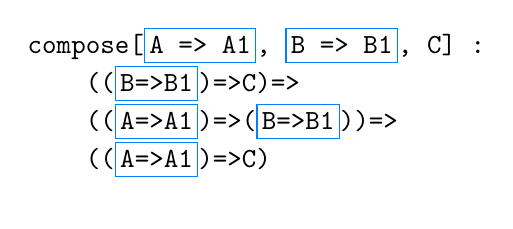
\begin{tikzpicture}[remember picture]
            \codeBlock{
            compose[\cPart{a1}{A => A1}, \cPart{b1}{B => B1}, C] :\\
            \ptab{}((\cPart{b2}{B=>B1})=>C)=>\\
            \ptab{}((\cPart{a2}{A=>A1})=>(\cPart{b3}{B=>B1}))=>\\
            \ptab{}((\cPart{a2}{A=>A1})=>C)\\
            }
        \end{tikzpicture}
    \end{frame}

\end{document}